\documentclass[journal,12pt,twocolumn]{IEEEtran}
\usepackage[shortlabels]{enumitem}
\usepackage{setspace}
\usepackage{gensymb}
\singlespacing
\usepackage[cmex10]{amsmath}
\usepackage{graphicx}

\usepackage{float}
\usepackage{amsthm}

\usepackage{mathrsfs}
\usepackage{txfonts}
\usepackage{stfloats}
\usepackage{bm}
\usepackage{cite}
\usepackage{cases}
\usepackage{subfig}

\usepackage{longtable}
\usepackage{multirow}

\usepackage{enumitem}
\usepackage{mathtools}
\usepackage{steinmetz}
\usepackage{tikz}
\usepackage{circuitikz}
\usepackage{verbatim}
\usepackage{tfrupee}
\usepackage[breaklinks=true]{hyperref}
\usepackage{graphicx}
\usepackage{tkz-euclide}

\usetikzlibrary{calc,math}
\usepackage{listings}
    \usepackage{color}                                            %%
    \usepackage{array}                                            %%
    \usepackage{longtable}                                        %%
    \usepackage{calc}                                             %%
    \usepackage{multirow}                                         %%
    \usepackage{hhline}                                           %%
    \usepackage{ifthen}                                           %%
    \usepackage{lscape}     
\usepackage{multicol}
\usepackage{chngcntr}

\DeclareMathOperator*{\Res}{Res}

\renewcommand\thesection{\arabic{section}}
\renewcommand\thesubsection{\thesection.\arabic{subsection}}
\renewcommand\thesubsubsection{\thesubsection.\arabic{subsubsection}}

\renewcommand\thesectiondis{\arabic{section}}
\renewcommand\thesubsectiondis{\thesectiondis.\arabic{subsection}}
\renewcommand\thesubsubsectiondis{\thesubsectiondis.\arabic{subsubsection}}


\hyphenation{op-tical net-works semi-conduc-tor}
\def\inputGnumericTable{}                                 %%

\lstset{
%language=C,
frame=single, 
breaklines=true,
columns=fullflexible
}
\begin{document}

\newcommand{\BEQA}{\begin{eqnarray}}
\newcommand{\EEQA}{\end{eqnarray}}
\newcommand{\define}{\stackrel{\triangle}{=}}
\bibliographystyle{IEEEtran}
\raggedbottom
\setlength{\parindent}{0pt}
\providecommand{\mbf}{\mathbf}
\providecommand{\pr}[1]{\ensuremath{\Pr\left(#1\right)}}
\providecommand{\qfunc}[1]{\ensuremath{Q\left(#1\right)}}
\providecommand{\sbrak}[1]{\ensuremath{{}\left[#1\right]}}
\providecommand{\lsbrak}[1]{\ensuremath{{}\left[#1\right.}}
\providecommand{\rsbrak}[1]{\ensuremath{{}\left.#1\right]}}
\providecommand{\brak}[1]{\ensuremath{\left(#1\right)}}
\providecommand{\lbrak}[1]{\ensuremath{\left(#1\right.}}
\providecommand{\rbrak}[1]{\ensuremath{\left.#1\right)}}
\providecommand{\cbrak}[1]{\ensuremath{\left\{#1\right\}}}
\providecommand{\lcbrak}[1]{\ensuremath{\left\{#1\right.}}
\providecommand{\rcbrak}[1]{\ensuremath{\left.#1\right\}}}
\theoremstyle{remark}
\newtheorem{rem}{Remark}
\newcommand{\sgn}{\mathop{\mathrm{sgn}}}
\providecommand{\abs}[1]{\vert#1\vert}
\providecommand{\res}[1]{\Res\displaylimits_{#1}} 
\providecommand{\norm}[1]{\lVert#1\rVert}
%\providecommand{\norm}[1]{\lVert#1\rVert}
\providecommand{\mtx}[1]{\mathbf{#1}}
\providecommand{\mean}[1]{E[ #1 ]}
\providecommand{\fourier}{\overset{\mathcal{F}}{ \rightleftharpoons}}
%\providecommand{\hilbert}{\overset{\mathcal{H}}{ \rightleftharpoons}}
\providecommand{\system}{\overset{\mathcal{H}}{ \longleftrightarrow}}
	%\newcommand{\solution}[2]{\textbf{Solution:}{#1}}
\newcommand{\solution}{\noindent \textbf{Solution: }}
\newcommand{\cosec}{\,\text{cosec}\,}
\providecommand{\dec}[2]{\ensuremath{\overset{#1}{\underset{#2}{\gtrless}}}}
\newcommand{\myvec}[1]{\ensuremath{\begin{pmatrix}#1\end{pmatrix}}}
\newcommand{\mydet}[1]{\ensuremath{\begin{vmatrix}#1\end{vmatrix}}}
\numberwithin{equation}{subsection}
\makeatletter
\@addtoreset{figure}{problem}
\makeatother
\let\StandardTheFigure\thefigure
\let\vec\mathbf
\renewcommand{\thefigure}{\theproblem}
\def\putbox#1#2#3{\makebox[0in][l]{\makebox[#1][l]{}\raisebox{\baselineskip}[0in][0in]{\raisebox{#2}[0in][0in]{#3}}}}
     \def\rightbox#1{\makebox[0in][r]{#1}}
     \def\centbox#1{\makebox[0in]{#1}}
     \def\topbox#1{\raisebox{-\baselineskip}[0in][0in]{#1}}
     \def\midbox#1{\raisebox{-0.5\baselineskip}[0in][0in]{#1}}
\vspace{3cm}
\title{AI1103-Assignment-3}
\author{Kodavanti Rama Sravanth,CS20BTECH11027}
\maketitle
\newpage
\bigskip
\renewcommand{\thefigure}{\theenumi}
\renewcommand{\thetable}{\theenumi}
Download all python codes from 
\begin{lstlisting}
https://github.com/Sravanth-k27/AI1103/tree/main/Assignment-3/codes
\end{lstlisting}
%
Download latex-tikz codes from 
%
\begin{lstlisting}
 https://github.com/Sravanth-k27/AI1103/tree/main/Assignment-3/Assignment-3.tex 
\end{lstlisting}
\section*{Question:Gate 2012 (MA) ,Q.29}
If a random variable X assumes only positive integral values ,with the probability
\begin{equation}
 P(X=x)=\frac{2}{3}\brak{\frac{1}{3}}^{x-1},x=1,2,3,....,   
\end{equation}

then $E(X)$ is 
\begin{enumerate}[(A)]
\begin{multicols}{2}
\item $ \frac{2}{9}$\\
\item $\frac{2}{3}$\\
\item $ 1$\\
\item $\frac{3}{2}$
\end{multicols}
\end{enumerate}
\section*{Solution:Gate 2012 (MA) ,Q.29}
  Given that random variable X  assumes only positive integral values and its probability is:
  \begin{align}
      P(X=x)=\frac{2}{3}\brak{\frac{1}{3}}^{x-1}
  \end{align}
  The expectation value E(X) is given by 
  \begin{align}
      E(X)=\sum_{i=1}^{\infty} i \times P(X=i)
  \end{align}
  Let $E(X)=S$\\
  so,
  \begin{align}
      S&=\sum_{i=1}^{\infty} i \times P(X=i)\\
    \implies S&=\sum_{i=1}^{\infty} i \times
      \frac{2}{3}\brak{\frac{1}{3}}^{i-1}\label{eq:0.0.5}\\
     \implies S&=\frac{2}{3}+\sum_{i=2}^{\infty} i \times
      \frac{2}{3}\brak{\frac{1}{3}}^{i-1}\label{eq:0.0.6}
  \end{align}
  As
  \begin{align}
      \sum_{i=2}^{\infty} i \times
      \frac{2}{3}\brak{\frac{1}{3}}^{i-1}=\sum_{i=1}^{\infty} (i+1)\times
      \frac{2}{3}\brak{\frac{1}{3}}^{i}\label{eq:0.0.7}
  \end{align}
  Now substituting  \eqref{eq:0.0.7} in \eqref{eq:0.0.6}
  \begin{align}
      \implies S&=\frac{2}{3}+\sum_{i=1}^{\infty} (i+1) \times
      \frac{2}{3}\brak{\frac{1}{3}}^{i}
  \end{align}
  \begin{align}
       \implies S&=\frac{2}{3}+\sum_{i=1}^{\infty} i \times
      \frac{2}{3}\brak{\frac{1}{3}}^{i}+\sum_{i=1}^{\infty} 
      \frac{2}{3}\brak{\frac{1}{3}}^{i}\label{eq:0.0.9}
  \end{align}
   Dividing with 3 on both sides in \eqref{eq:0.0.5} gives
   \begin{align}
      \frac{S}{3}=\sum_{i=1}^{\infty} i \times
      \frac{2}{3}\brak{\frac{1}{3}}^{i}\label{eq:0.0.10}
  \end{align}
  Now substituting \eqref{eq:0.0.10} in \eqref{eq:0.0.9} gives
  \begin{align}
     \implies S&=\frac{2}{3}+\frac{S}{3}+\sum_{i=1}^{\infty}\frac{2}{3}\brak{\frac{1}{3}}^{i}
     \end{align}
     \begin{align}
     \implies \frac{2S}{3}&=\frac{2}{3}+\frac{2}{3}\sum_{i=1}^{\infty}\brak{\frac{1}{3}}^{i}
  \end{align}
  \begin{align}
     \implies \frac{2S}{3}&=\frac{2}{3}\brak{
     1+\sum_{i=1}^{\infty}\brak{\frac{1}{3}}^{i}}
  \end{align}
  \begin{align}
     \implies S=1+\sum_{i=1}^{\infty}\brak{\frac{1}{3}}^{i}
  \end{align}
  \begin{align}
     \implies S=1+\frac{\frac{1}{3}}{1-\frac{1}{3}}
  \end{align}
  \begin{align}
     \implies S=1+\frac{1}{2}=\frac{3}{2}
  \end{align}
  \begin{align}
     \implies E(X)=S=\frac{3}{2}
  \end{align}
  \begin{center}
  \textbf{$\therefore$ Option D is correct}    
  \end{center}
\begin{figure}[h]
    \begin{center}
    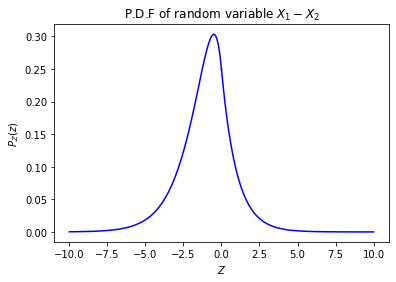
\includegraphics[scale=0.6,]{figure-1.png}
    \end{center}
    \caption{Theory vs simulated of P(X=x)}
    \label{fig:1}
\end{figure}

\end{document}
